% Options for packages loaded elsewhere
\PassOptionsToPackage{unicode}{hyperref}
\PassOptionsToPackage{hyphens}{url}
%
\documentclass[
]{article}
\usepackage{lmodern}
\usepackage{amsmath}
\usepackage{ifxetex,ifluatex}
\ifnum 0\ifxetex 1\fi\ifluatex 1\fi=0 % if pdftex
  \usepackage[T1]{fontenc}
  \usepackage[utf8]{inputenc}
  \usepackage{textcomp} % provide euro and other symbols
  \usepackage{amssymb}
\else % if luatex or xetex
  \usepackage{unicode-math}
  \defaultfontfeatures{Scale=MatchLowercase}
  \defaultfontfeatures[\rmfamily]{Ligatures=TeX,Scale=1}
\fi
% Use upquote if available, for straight quotes in verbatim environments
\IfFileExists{upquote.sty}{\usepackage{upquote}}{}
\IfFileExists{microtype.sty}{% use microtype if available
  \usepackage[]{microtype}
  \UseMicrotypeSet[protrusion]{basicmath} % disable protrusion for tt fonts
}{}
\makeatletter
\@ifundefined{KOMAClassName}{% if non-KOMA class
  \IfFileExists{parskip.sty}{%
    \usepackage{parskip}
  }{% else
    \setlength{\parindent}{0pt}
    \setlength{\parskip}{6pt plus 2pt minus 1pt}}
}{% if KOMA class
  \KOMAoptions{parskip=half}}
\makeatother
\usepackage{xcolor}
\IfFileExists{xurl.sty}{\usepackage{xurl}}{} % add URL line breaks if available
\IfFileExists{bookmark.sty}{\usepackage{bookmark}}{\usepackage{hyperref}}
\hypersetup{
  hidelinks,
  pdfcreator={LaTeX via pandoc}}
\urlstyle{same} % disable monospaced font for URLs
\usepackage{longtable,booktabs}
\usepackage{calc} % for calculating minipage widths
% Correct order of tables after \paragraph or \subparagraph
\usepackage{etoolbox}
\makeatletter
\patchcmd\longtable{\par}{\if@noskipsec\mbox{}\fi\par}{}{}
\makeatother
% Allow footnotes in longtable head/foot
\IfFileExists{footnotehyper.sty}{\usepackage{footnotehyper}}{\usepackage{footnote}}
\makesavenoteenv{longtable}
\usepackage{graphicx}
\makeatletter
\def\maxwidth{\ifdim\Gin@nat@width>\linewidth\linewidth\else\Gin@nat@width\fi}
\def\maxheight{\ifdim\Gin@nat@height>\textheight\textheight\else\Gin@nat@height\fi}
\makeatother
% Scale images if necessary, so that they will not overflow the page
% margins by default, and it is still possible to overwrite the defaults
% using explicit options in \includegraphics[width, height, ...]{}
\setkeys{Gin}{width=\maxwidth,height=\maxheight,keepaspectratio}
% Set default figure placement to htbp
\makeatletter
\def\fps@figure{htbp}
\makeatother
\setlength{\emergencystretch}{3em} % prevent overfull lines
\providecommand{\tightlist}{%
  \setlength{\itemsep}{0pt}\setlength{\parskip}{0pt}}
\setcounter{secnumdepth}{-\maxdimen} % remove section numbering
\ifluatex
  \usepackage{selnolig}  % disable illegal ligatures
\fi

\author{}
\date{}

\begin{document}

\hypertarget{rapport-danalyse-de-besoin}{%
\section{Rapport d'analyse de besoin}\label{rapport-danalyse-de-besoin}}

\begin{center}\rule{0.5\linewidth}{0.5pt}\end{center}

\underline{\textbf{Sommaire}}

\tableofcontents

\hypertarget{introduction}{%
\subsection{Introduction}\label{introduction}}

\begin{enumerate}
\def\labelenumi{\arabic{enumi}.}
\item
  \textbf{Contexte générale:}
\end{enumerate}

Dans le cadre de la modernisation de la gestion des secteurs publics
collectifs marocains, l'état a créé des contrats de gestion déléguées.
Parmi ces dernières, les contrats de gestion de transport urbain. Ainsi
l'état a pris ce sens pour réaliser ses objectifs d'ouverture sur
l'économie mondiale, le soutien des entreprises publiques, et
l'amélioration de ses services. En parallèle avec ceci, l'état a essayé
de gagner les défis de la régionalisation. Par conséquent, la gestion et
le suivis des contrats de transport a devenu une tâche fondamentale. Or,
effectuer cette tâche d'une manière classique est fastidieuse, vue le
nombre de lecture et de vérification des données importantes dans les
documents nombreux. En plus, cela ne permet pas d'en tirer profits pour
prendre les bons décisions facilement. Ainsi, nous proposons une
solution simple pour la gestion et la représentation des données en
question.

\begin{enumerate}
\def\labelenumi{\arabic{enumi}.}
\item
  \textbf{Définitions et Problématique:}
\end{enumerate}

Les contrats de gestion déléguée du transport urbain comportent
plusieurs actes qui forment un ensemble de règles à respecter entre un
délégant qui sont une ou plusieurs communes et un délégataire qui est
une société. En addition, des pénalités sont imposer en cas de non
respect des règles posées dans le contrat. D'où l'importance d'avoir des
données bien présentées pour faire le suivi et veiller sur le respect
des conditions prédéfinis. Ceci s'intègre dans le cadre de la bon
gestion de territoire et des aménagements publics.

\begin{enumerate}
\def\labelenumi{\arabic{enumi}.}
\item
  \textbf{Objectifs:}
\end{enumerate}

On cherche à concevoir et construire une solution qui permet de saisir,
d'enregistrer, et de traiter les données qui concernent les contrats de
gestion de transport. La solution proposée est composée de deux partie:
une première partie qui concerne la saisi et l'enregistrement des
données sous la forme d'une plateforme web liée à une base de donné, et
une deuxième partie qui concerne l'analyse des données.

Bref, on cherche une solution pour:

\begin{itemize}
\item
  Centraliser l'information contenue dans les contrats de gestion
  déléguée et leurs avenants le cas échéant .
\item
  Centraliser les documents exigés par le contrat que l'opérateur est
  tenu de fournir périodiquement à l'autorité délégante.
\item
  Permettre aux utilisateurs de partager en interne des informations et
  des documents.
\item
  Assurer le suivi de la gestion des contrats de transport urbain.
\end{itemize}

\hypertarget{planification}{%
\subsection{Planification}\label{planification}}

\begin{enumerate}
\def\labelenumi{\arabic{enumi}.}
\item
  \textbf{Plan général:}
\end{enumerate}

Pour la bonne organisation des étapes du projets, nous proposons
premièrement le plan suivant pour la réalisation de la plateforme:

\begin{figure}
\centering
\includegraphics[width=10.83333in,height=\textheight]{16290405093251.png}
\caption{}
\end{figure}

\begin{enumerate}
\def\labelenumi{\arabic{enumi}.}
\item
  \textbf{Définition des Livrables:}
\end{enumerate}

À la fin de chaque étape de la réalisation (section dans le diagramme de
Gantt si-dessus), il est exigé d'avoir un livrable. Les livrables que
nous proposons sont les suivants:

\begin{longtable}[]{@{}ll@{}}
\toprule
Étape & Livrable\tabularnewline
\midrule
\endhead
Analyse & \emph{Document de spécification} décrivant le besoin, les
fonctionnalités de la solution à implémenter, les technologies à
utiliser, et toutes les contraints à respecter dans le
projet\tabularnewline
Conception & \emph{Document de conception} qui donne une idée clair et
global sur le projet\tabularnewline
Réalisation & \emph{plateforme de suivi} de l'exécution des Contrats de
Gestion de mobilité Urbaine\tabularnewline
\bottomrule
\end{longtable}

\begin{enumerate}
\def\labelenumi{\arabic{enumi}.}
\item
  \textbf{Mode de travail:}
\end{enumerate}

Afin de réaliser le projet, on doit définir un mode de travail
convenable. Le mode de travail que nous proposons est le mode
\emph{agile} en utilisant \emph{SCRUM}. Puisque nous travail dans un
environnement où on garde un contact continue avec le \emph{Product
Owner}. En plus, nous cherchons à avoir une communication efficace avec
le client pour le satisfaire en lui livrant fréquemment une application
utilisable rapidement. D'ailleurs, le temps est un facteur important
dans notre projet, pour ceci il faut sentir l'avancement quotidienne du
projet. En addition, il faut faire attention continue à l'excellence
technique, à une meilleure conception et produire uniquement ce qui est
nécessaire dans les meilleurs délais. Ainsi, on présente le tableau
suivant basée sur le modèle kanban pour l'organisation des tâches et des
livrables:

\begin{figure}
\centering
\includegraphics{/home/kotbi/Documents/EnsiasRessources/modèle kanban.png}
\caption{}
\end{figure}

\hypertarget{analyse}{%
\subsection{Analyse}\label{analyse}}

\begin{enumerate}
\def\labelenumi{\arabic{enumi}.}
\item
  \textbf{Analyse fonctionnelle:}

  \begin{itemize}
  \item
    \textbf{Description générale du projet:}

    Le projet est décomposé en trois partie. La première concernant la
    partie client dans laquelle l'utilisateur peut saisir les données.
    Ensuite, une base de données \texttt{SQL\ server} et enfin la partie
    reporting.

    \begin{figure}
    \centering
    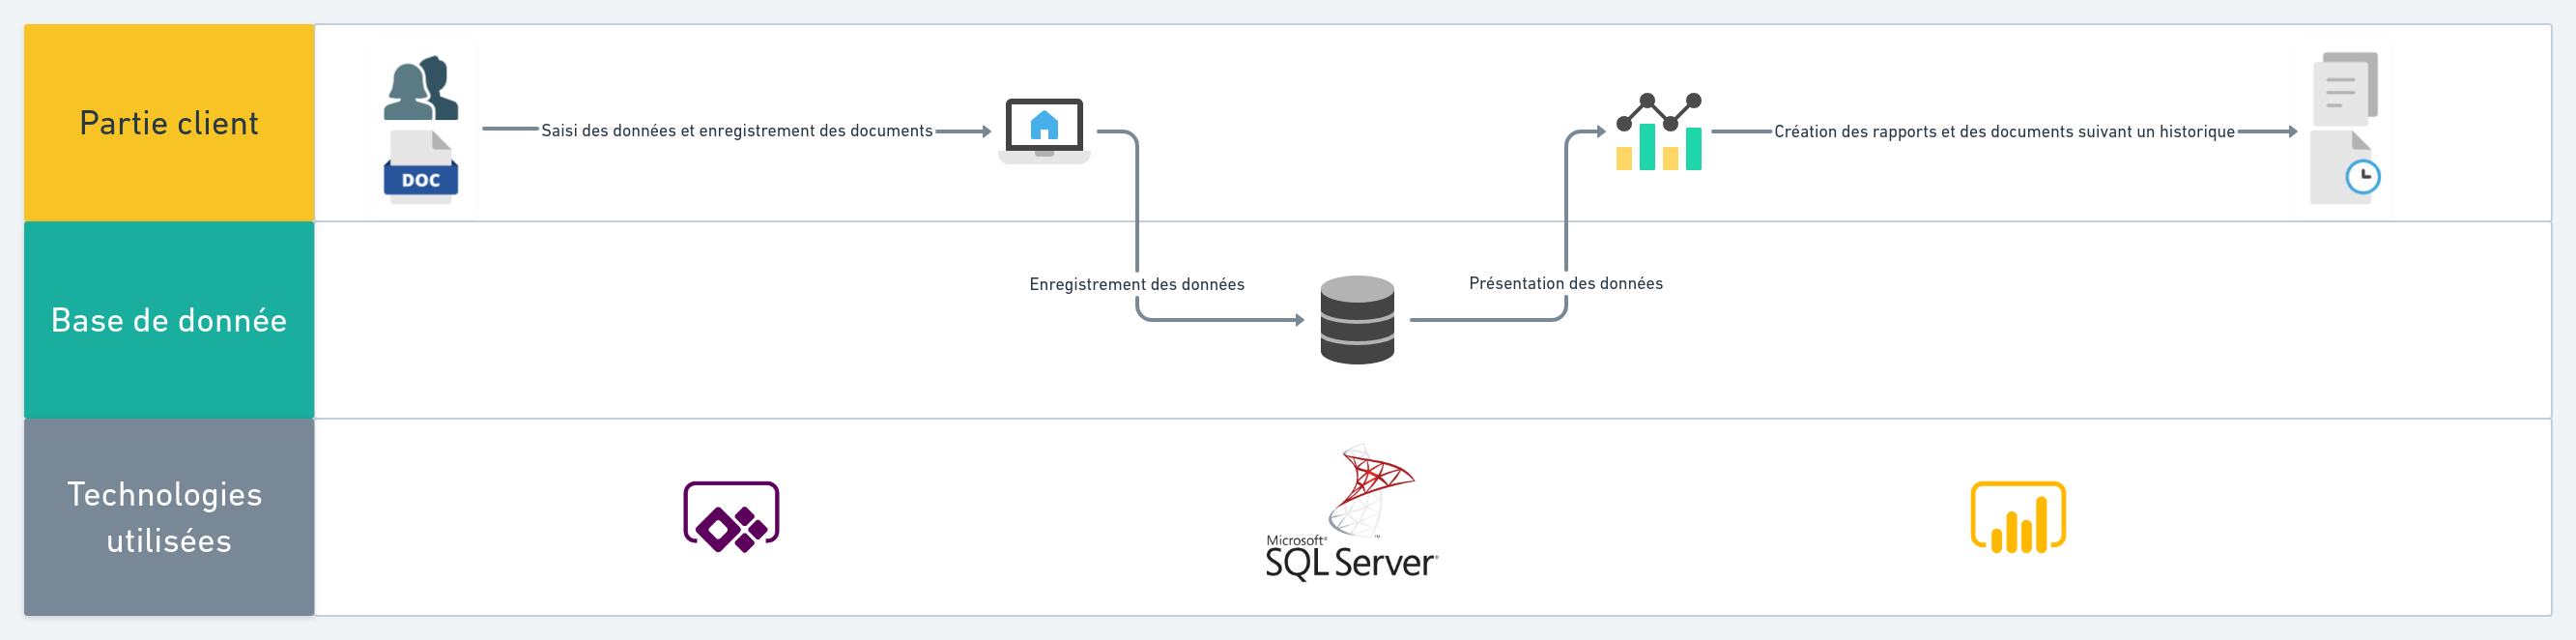
\includegraphics{/home/kotbi/Documents/EnsiasRessources/KDI.png}
    \caption{}
    \end{figure}
  \item
    \textbf{Analyse de l'existant:}

    Nous avons effectué une recherche sur des applications similaires.
    Généralement se sont des applications qui aide à la gestion de
    donnée et des ressources, et la prise des décisions. L'application
    \emph{Environnement Canterbury} (ECan) fait partie du gouvernement
    local de la région de Canterbury en Nouvelle-Zélande. Ils ont
    utilisé la plate-forme Power (PowerApps, Microsoft Flow et Power BI)
    pour gérer et rendre compte efficacement des projets d'eau douce et
    de ressources naturelles.

    D'après l'article intitulé
    \href{https://powerapps.microsoft.com/fr-fr/blog/environment-canterbury-speeds-up-outcome-tracking-with-the-power-platform/}{Environnement
    Canterbury accélère le suivi des résultats avec la Power Platform} :

    \emph{"Environnement Canterbury travaille en partenariat avec les
    communautés de Canterbury pour promouvoir la gestion durable des
    ressources naturelles. Cela implique l'utilisation de méthodes
    innovantes, rentables et techniquement excellentes, et garantit que
    la prise de décision est basée sur des informations de la plus haute
    qualité. Ils travaillent sur des programmes de résultats
    environnementaux à long terme qui consistent en plusieurs étapes et
    projets connexes. ECan avait besoin d'une solution abordable qui
    offrirait une plus grande cohérence entre les projets, des niveaux
    de visibilité plus élevés et un accès plus rapide aux données."}

    \begin{figure}
    \centering
    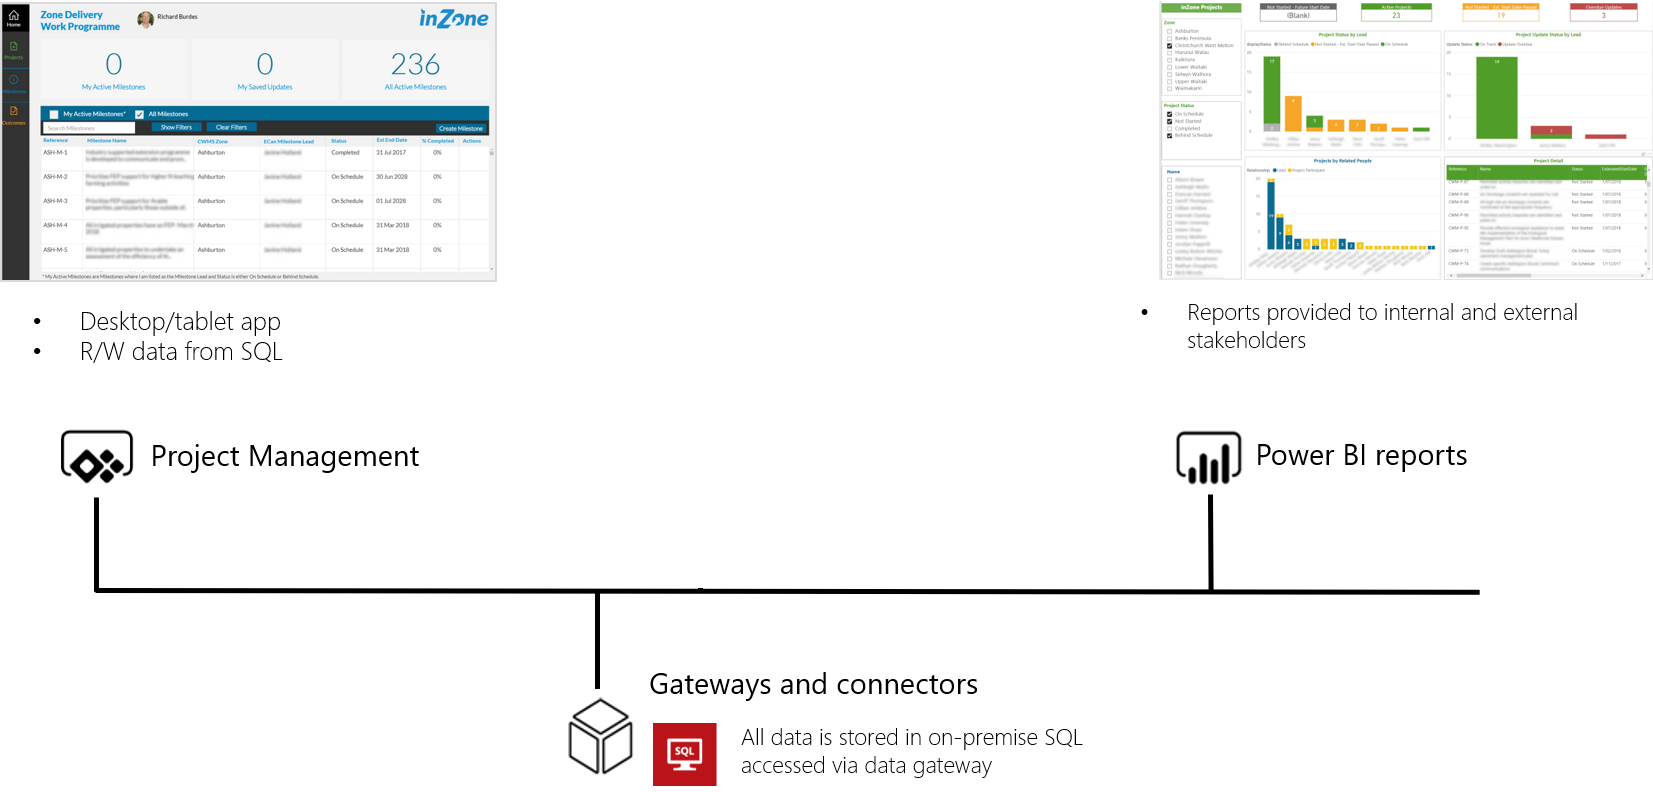
\includegraphics{/home/kotbi/Documents/EnsiasRessources/example.png}
    \caption{}
    \end{figure}
  \item
    \textbf{WBS:}

    Suivant à ce qui précède et d'après les documents communiqués, nous
    avons essayé de créer une décomposition hiérarchique orientée
    livrable du projet.

    \begin{figure}
    \centering
    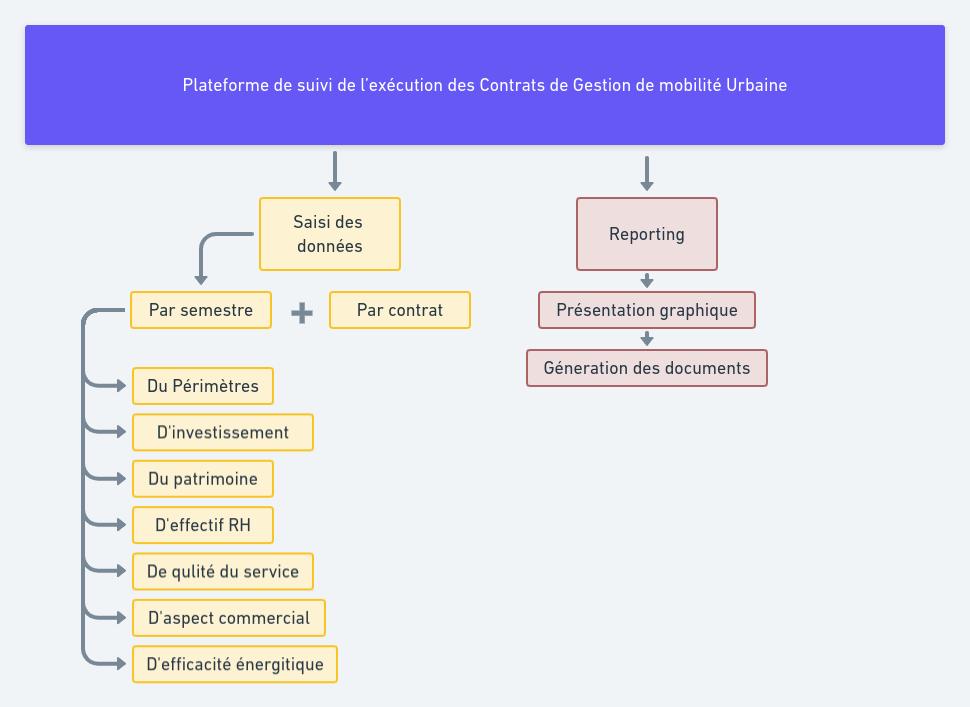
\includegraphics{/home/kotbi/Documents/EnsiasRessources/WBS KPI.png}
    \caption{}
    \end{figure}
  \end{itemize}

  \begin{itemize}
  \item
    \textbf{Analyse de données}:

    La solution que nous proposons est une solution basée sur les
    données. Autrement dite, elle permet à son utilisateur d'interagir
    avec plusieurs informations. En outre, elle représente une solution
    spécialisée pour l'acquisition, la gestion et la présentation
    d'informations. Donc il faut bien comprendre les relations entre les
    données et comment elle doivent être traitées. Pour le faire, on
    propose le dictionnaire des données suivant:

    \begin{longtable}[]{@{}lll@{}}
    \toprule
    Table Contrat & &\tabularnewline
    \midrule
    \endhead
    \textbf{Attribut} & \textbf{Signification} &
    \textbf{Exemple}\tabularnewline
    IDCont & Identificateur du contrat & 11\tabularnewline
    DateVisa & Date visa & 26-Jul-13\tabularnewline
    IDAvenantActif & Identificateur de l'avenant actif &
    20\tabularnewline
    Titre & titre du contrat & gestion deleguee de
    transport\tabularnewline
    IDDelegant & Identificateur du délégant & la commune de
    tanger\tabularnewline
    IDDelegataire & Identificateur du délégataire & Societe ALSA
    TANGER\tabularnewline
    \bottomrule
    \end{longtable}

    \begin{longtable}[]{@{}lll@{}}
    \toprule
    Table Avenant & &\tabularnewline
    \midrule
    \endhead
    \textbf{Attribut} & \textbf{Signification} &
    \textbf{Exemple}\tabularnewline
    IDAvenant & Identificateur de l'avenant & 20\tabularnewline
    Date & & 1-Jun-14\tabularnewline
    Motif & &\tabularnewline
    IDCont & Identificateur du contrat & 11\tabularnewline
    Duree & & 10 ans\tabularnewline
    Status & si l'avenent est actif ou non & actif\tabularnewline
    NombreCommunes & Nombre de communes desservis & 15\tabularnewline
    Population & & 1 105 783 Habt\tabularnewline
    LonguerReseau & Longueur du réseau & 849,4 Km\tabularnewline
    NombreLignes & & 45 lignes\tabularnewline
    LLUrbaines & Longueur des lignes urbaines & 315,4 Km\tabularnewline
    LLPeripheriques & Longueur des lignes périphériques & 534
    Km\tabularnewline
    \bottomrule
    \end{longtable}

    \begin{longtable}[]{@{}lll@{}}
    \toprule
    Table Révision & &\tabularnewline
    \midrule
    \endhead
    \textbf{Attribut} & \textbf{Signification} &
    \textbf{Exemple}\tabularnewline
    IDRevision & Identificateur de révision & 30\tabularnewline
    Date & & En cours\tabularnewline
    Motif & & Parc inssufisant et déséquilibre du contrat\tabularnewline
    IDAven & Identificateur de l'avenant & 20\tabularnewline
    \bottomrule
    \end{longtable}

    \begin{longtable}[]{@{}lll@{}}
    \toprule
    Table Délégataire & &\tabularnewline
    \midrule
    \endhead
    \textbf{Attribut} & \textbf{Signification} &
    \textbf{Exemple}\tabularnewline
    IDDelegataire & Identificateur du délégataire & 40\tabularnewline
    Nom & Nom du délégataire & Societe ALSA TANGER\tabularnewline
    \bottomrule
    \end{longtable}

    \begin{longtable}[]{@{}lll@{}}
    \toprule
    Table Délégant & &\tabularnewline
    \midrule
    \endhead
    \textbf{Attribut} & \textbf{Signification} &
    \textbf{Exemple}\tabularnewline
    IDDeleguant & Identificateur du délégant & 50\tabularnewline
    Nom & nom du délégant & la commune de tanger\tabularnewline
    IDCommune & Identificateur de la commune & 60\tabularnewline
    \bottomrule
    \end{longtable}

    \begin{longtable}[]{@{}lll@{}}
    \toprule
    Table Commune & &\tabularnewline
    \midrule
    \endhead
    \textbf{Attribut} & \textbf{Signification} &
    \textbf{Exemple}\tabularnewline
    IDCommune & Identificateur de la commune & 60\tabularnewline
    Nom & nom de la commune & la commune de tanger\tabularnewline
    \bottomrule
    \end{longtable}

    \begin{longtable}[]{@{}lll@{}}
    \toprule
    Table Tarifs & &\tabularnewline
    \midrule
    \endhead
    \textbf{Attribut} & \textbf{Signification} &
    \textbf{Exemple}\tabularnewline
    IDTarif & Identificateur du tarif & 70\tabularnewline
    IDAven & Identificateur de l'avenant & 20\tabularnewline
    Description & une description du tarif & tarif normale: ticket
    réseau urbain\tabularnewline
    Valeurs & les valeurs du tarif & 2,5DH 3,5 DH\tabularnewline
    Annee & & 2014\tabularnewline
    Periode & Semestre & T1\tabularnewline
    \bottomrule
    \end{longtable}

    \begin{longtable}[]{@{}lll@{}}
    \toprule
    Table EffectifPersonnel & &\tabularnewline
    \midrule
    \endhead
    \textbf{Attribut} & \textbf{Signification} &
    \textbf{Exemple}\tabularnewline
    IDEP & Identificateur de l'effectif personnel & 80\tabularnewline
    IDAven & Identificateur de l'avenant & 20\tabularnewline
    Profil & Profil du personnel & Conducteur\tabularnewline
    Periode & semestre & T1\tabularnewline
    Annee & & 2014\tabularnewline
    \bottomrule
    \end{longtable}

    \begin{longtable}[]{@{}lll@{}}
    \toprule
    Table Investissement & &\tabularnewline
    \midrule
    \endhead
    \textbf{Attribut} & \textbf{Signification} &
    \textbf{Exemple}\tabularnewline
    IDInvst & Identificateur de l'investissement & 90\tabularnewline
    Description & Desciption de l'investissement & Bus
    touristique\tabularnewline
    Type & Type de l'investissement (contractuel ou réalisé) &
    contractuel\tabularnewline
    Valeur & la valeur de l'investissement & 184,131,445\tabularnewline
    Periode & semestre & T1\tabularnewline
    Annee & & 2014\tabularnewline
    Partenaire & & Partemaire\tabularnewline
    \bottomrule
    \end{longtable}

    \begin{longtable}[]{@{}lll@{}}
    \toprule
    Table MaterielCirculant & &\tabularnewline
    \midrule
    \endhead
    \textbf{Attribut} & \textbf{Signification} &
    \textbf{Exemple}\tabularnewline
    IDMatCirculant & Identificateur du materiel circulant &
    100\tabularnewline
    Nombre & & 59\tabularnewline
    AgeMoyen & & 6,68 ans\tabularnewline
    Kmparcourus & & 88,361,937\tabularnewline
    Periode & semestre & T2\tabularnewline
    Annee & & 2015\tabularnewline
    Description & & Bus standard\tabularnewline
    IDAven & Identificateur de l'avenant & 20\tabularnewline
    \bottomrule
    \end{longtable}

    \begin{longtable}[]{@{}lll@{}}
    \toprule
    Table MaterielFixe & &\tabularnewline
    \midrule
    \endhead
    \textbf{Attribut} & \textbf{Signification} &
    \textbf{Exemple}\tabularnewline
    IDMatFixe & Identificateur du materiel fixe & 200\tabularnewline
    Periode & semestre & T3\tabularnewline
    Annee & & 2015\tabularnewline
    Nombre & & 2\tabularnewline
    AgeMoyen & & 7 ans\tabularnewline
    Capacite Totale & & 198 places\tabularnewline
    Description & & Aires de stationnement\tabularnewline
    IDAven & Identificateur de l'avenant & 20\tabularnewline
    \bottomrule
    \end{longtable}

    \begin{longtable}[]{@{}lll@{}}
    \toprule
    Table QualiteService & &\tabularnewline
    \midrule
    \endhead
    \textbf{Attribut} & \textbf{Signification} &
    \textbf{Exemple}\tabularnewline
    IDQS & Identificateur du qualité de service & 300\tabularnewline
    IDAven & Identificateur de l'avenant & 20\tabularnewline
    Periode & semestre & T1\tabularnewline
    Annee & & 2016\tabularnewline
    PQM & Plan du maintenance Qualité & oui\tabularnewline
    Reclamation & Réclamation des usagers & 22/semestre\tabularnewline
    Equipement & Equipement des points d'arrêt & Signalisation
    verticale: abrisbus, poteaux d'arret\tabularnewline
    SAEV & Système d'information de type SAEV(Système d'aide à
    l'exploitation et à l'information voyageurs) & OUI\tabularnewline
    SYSGeo & Système de géolocalisation & oui\tabularnewline
    WifiEmb & wifi embarqué & non\tabularnewline
    VedioSurvEmb & video surveillance embarquée & oui\tabularnewline
    CentreAppel & centre d'appel & non\tabularnewline
    Adresse & & oui\tabularnewline
    InfoStatReseau & Informations statiques sur le réseau &
    oui\tabularnewline
    HoraireServ & horaires du service & oui\tabularnewline
    InfosPertu & informations sur les perturbations & non\tabularnewline
    TarifsApp & Tarifs appliqués & oui\tabularnewline
    VenteEnLigne & & non\tabularnewline
    Correspondances & & oui\tabularnewline
    Intermodalité & & oui\tabularnewline
    \bottomrule
    \end{longtable}

    \begin{longtable}[]{@{}lll@{}}
    \toprule
    Table AspectComm(commercial) & &\tabularnewline
    \midrule
    \endhead
    \textbf{Attribut} & \textbf{Signification} &
    \textbf{Exemple}\tabularnewline
    IDAC & Identificateur del'aspect commercial & 400\tabularnewline
    IDAven & Identificateur de l'avenant & 20\tabularnewline
    NbrVoyJrs & nombre de voyageur par jours & 117,442\tabularnewline
    NbrPlaceVidJrs & nombre de places vides par jours &
    283\tabularnewline
    TotAnnVoyJrs & Total annuel de voyageur par jours &
    24,662,833\tabularnewline
    TicketsVendu & Nombre de tickets svendu & 37,781,318\tabularnewline
    Kmparcourus & & 8 018 629 Km\tabularnewline
    FreqMoyPass & fréquence moyenne de passage & 1.33
    passage/jours\tabularnewline
    VitesseComm & vitesse commerciale moyenne & 17
    Km/heure\tabularnewline
    Ponctualité & & 9 min\tabularnewline
    TauxRempli & Taux de remplissage & 71.92\%\tabularnewline
    HeurDepartServ & heure de départ de service & 4:45H\tabularnewline
    HeureFinServ & Heure de fin de service & 22:45H\tabularnewline
    Pannes & nombre de pannes & 6500\tabularnewline
    Accidents & nombre d'accidents & 511\tabularnewline
    DelaiMoyEvacu & Delai moyen d'évacuation & 15 min\tabularnewline
    Période & semestre & T3\tabularnewline
    Annee & & 2016\tabularnewline
    \bottomrule
    \end{longtable}

    \begin{longtable}[]{@{}lll@{}}
    \toprule
    Table d'efficaciteEnergitiqueMoyenne & &\tabularnewline
    \midrule
    \endhead
    \textbf{Attribut} & \textbf{Signification} &
    \textbf{Exemple}\tabularnewline
    IDEffEnMoy & Identificateur d'éfficacité énergitique &
    500\tabularnewline
    IDAven & Identificateur de l'avenant & 20\tabularnewline
    ConsomationCarbu & la consomation du carburant & 4 616.72
    Tonnes\tabularnewline
    ConsomationTotalElec & la consomation total en électricité & 490
    996.47 KWH\tabularnewline
    EmmissionCarb & Emission du carbone CO2 & 14 055
    Tonnes\tabularnewline
    Periode & semestre & T2\tabularnewline
    Annee & & 2016\tabularnewline
    \bottomrule
    \end{longtable}

    \begin{longtable}[]{@{}lll@{}}
    \toprule
    Table d'efficaciteEnergitiqueTotal & &\tabularnewline
    \midrule
    \endhead
    \textbf{Attribut} & \textbf{Signification} &
    \textbf{Exemple}\tabularnewline
    IDEffEnTotal & Identificateur d'efficacite energitique total &
    600\tabularnewline
    IDAven & Identificateur de l'avenant & 20\tabularnewline
    ConsomationMoy & Consomation moyenne par Km et par type de bus &
    26.97 litres/100km\tabularnewline
    TypeMoyenTrans & Type du moyen de transport & minibus\tabularnewline
    Periode & semestre & T2\tabularnewline
    Annee & & 2016\tabularnewline
    \bottomrule
    \end{longtable}

    D'où on obtient le modèle conceptuel de données suivant:

    \begin{figure}
    \centering
    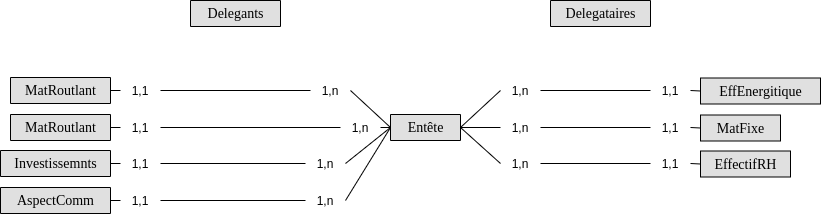
\includegraphics{/home/kotbi/Documents/EnsiasRessources/MCD.png}
    \caption{}
    \end{figure}

    Enfin nous proposons le schéma relationnel de la base de données
    suivant:

    \begin{figure}
    \centering
    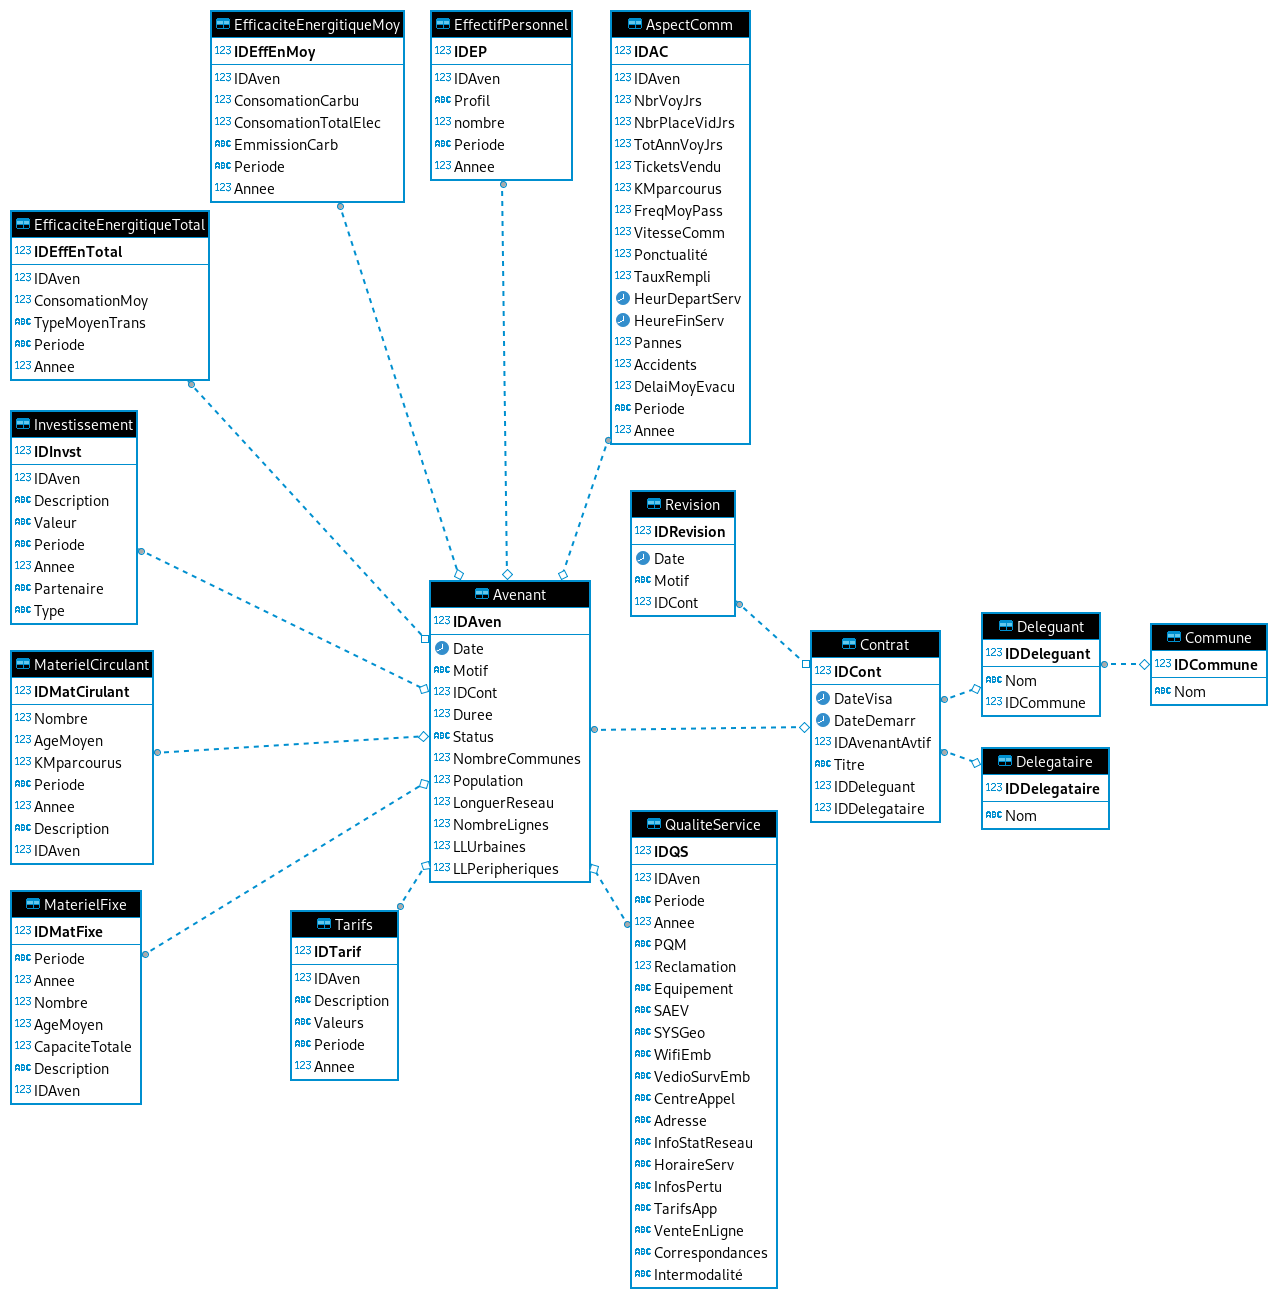
\includegraphics{/home/kotbi/Documents/EnsiasRessources/database.png}
    \caption{}
    \end{figure}
  \item
    \textbf{Maquettes(UI Design):}\\
    Pour bien comprendre un cas d'utilisation complet et parfait de
    l'application, et ainsi présenter toutes les pages de l'application,
    nous présentons le design
    suivant:\includegraphics{/home/kotbi/Documents/EnsiasRessources/KDI UI Design.png}
  \end{itemize}
\end{enumerate}

\begin{enumerate}
\def\labelenumi{\arabic{enumi}.}
\item
  \textbf{Analyse technique:}

  \begin{itemize}
  \item
    \textbf{Base de données:}
  \end{itemize}

  
\includegraphics{/home/kotbi/Documents/EnsiasRessources/outilsDB.png}\\
  \emph{Microsoft SQL Server} est un système de gestion de base de
  données relationnelle développé par Microsoft. En tant que serveur de
  base de données, il s'agit d'un produit logiciel dont la fonction
  principale est de stocker et de récupérer des données à la demande
  d'autres applications logicielles, qui peuvent s'exécuter sur le même
  ordinateur ou sur un autre ordinateur via un réseau.

  \begin{itemize}
  \item
    \textbf{Outils de développement:}
  \end{itemize}

  
\includegraphics{/home/kotbi/Documents/EnsiasRessources/outilsDEV.png}
  \\
  \emph{Power Apps} est un service permettant de créer et d'utiliser des
  applications professionnelles personnalisées qui se connectent à vos
  données et fonctionnent sur le Web et les appareils mobiles - sans le
  temps et les frais de développement de logiciels personnalisés.

  \begin{itemize}
  \item
    \textbf{Outils de reporting:}
  \end{itemize}

  
\includegraphics{/home/kotbi/Documents/EnsiasRessources/outilsREP.png}
  \\
  \emph{Power BI} est un service d'analyse commerciale de Microsoft. Il
  vise à fournir des visualisations interactives et des capacités de
  business intelligence avec une interface suffisamment simple pour que
  les utilisateurs finaux puissent créer leurs propres rapports et
  tableaux de bord. Il fait partie de la plate-forme Microsoft Power.

  \begin{itemize}
  \item
    \textbf{Gestion des fichiers:}

    La solution que nous proposons consiste à sauvegarder les fichiers
    sur un serveur WEB, et de sauvegarder en base de données le chemin
    de celui-ci. Généralement, cette solution est assez efficace, assez
    simple à mettre en oeuvre.
  \end{itemize}
\end{enumerate}

\hypertarget{ruxe9fuxe9rences}{%
\subsection{Références}\label{ruxe9fuxe9rences}}

\begin{itemize}
\item
  \href{https://trello.com/invite/b/QCUhh5sY/900fa738fc6c66193db04199e1248ae6/suivitransport}{Tableau
  Trello}
\item
  \href{https://whimsical.com/kdi-ux-design-J9PD866564ibwyMBwLHN9N}{Maquettes
  (UI design)}
\item
  \href{https://whimsical.com/wbs-kpi-9BDZ7oPFWEhvz9qQGoQEdL}{WBS}
\end{itemize}

\end{document}
